\newpage
\subsection*{Question 2}
\noindent [5 pts] Give a finite state automaton for the language denoted by the regular expression $r_1^*(r_2 + r_3)$, where $r_1 = a\emptyset a$, 
$r_2 = aa^*(a + b^*)$, and $r_3 = (b + ab)^*aa(b + ba)^*$.

\subsection*{Answer}
\noindent First, concerning $r_1 = a\emptyset a$, we know that with regular expressions, concatenating a string with an empty set always yields an empty set.
Since star closure is applied on that expression, it ends up being an empty character since $\emptyset ^* = \lambda$. In the context of this exercise $r_1$ 
can simply be ignored. \\

\noindent Then we have $r_2 = aa^*(a + b^*)$.
\noindent The corresponding NFA would be:
\begin{center}
    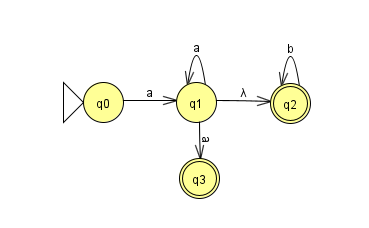
\includegraphics[width=0.4\textwidth]{img/graph1.png}
\end{center}

\noindent Finally we have $r_3 = (b + ab)^*aa(b + ba)^*$:

\begin{center}
    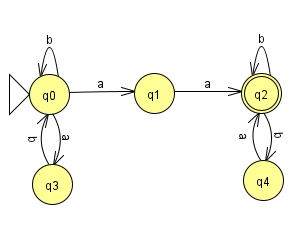
\includegraphics[width=0.3\textwidth]{img/graph2.png}
\end{center}

\noindent Now to obtain $(r_1 + r_2)$ we need to put both NFAs as two distinct path in a new NFA. We can obtain the following result:
\begin{center}
    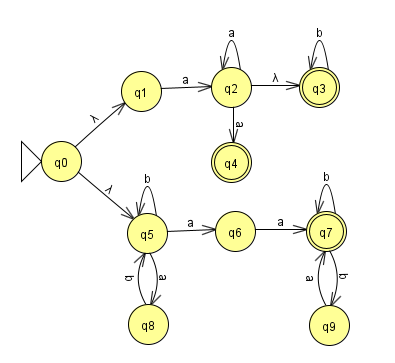
\includegraphics[width=0.4\textwidth]{img/graph3.png}
\end{center}


